%%%%%%%%%%%%%%%%%%%%%%%%%%%%%%%%%%%%%%%%%
% Short Sectioned Assignment
% LaTeX Template
% Version 1.0 (5/5/12)
%
% This template has been downloaded from:
% http://www.LaTeXTemplates.com
%
% Original author:
% Frits Wenneker (http://www.howtotex.com)
%
% License:
% CC BY-NC-SA 3.0 (http://creativecommons.org/licenses/by-nc-sa/3.0/)
%
%%%%%%%%%%%%%%%%%%%%%%%%%%%%%%%%%%%%%%%%%

%----------------------------------------------------------------------------------------
%	PACKAGES AND OTHER DOCUMENT CONFIGURATIONS
%----------------------------------------------------------------------------------------

\documentclass[paper=a4, fontsize=11pt]{scrartcl} % A4 paper and 11pt font size

\usepackage[T1]{fontenc} % Use 8-bit encoding that has 256 glyphs
\usepackage{fourier} % Use the Adobe Utopia font for the document - comment this line to return to the LaTeX default
\usepackage[spanish]{babel} % English language/hyphenation
\selectlanguage{spanish}
\usepackage[utf8]{inputenc}
\usepackage{amsmath,amsfonts,amsthm} % Math packages
\usepackage{graphicx}

\usepackage{sectsty} % Allows customizing section commands
\allsectionsfont{\centering \normalfont\scshape} % Make all sections centered, the default font and small caps

\usepackage{fancyhdr} % Custom headers and footers
\pagestyle{fancyplain} % Makes all pages in the document conform to the custom headers and footers
\date{}
\fancyhead{} % No page header - if you want one, create it in the same way as the footers below
\fancyfoot[L]{} % Empty left footer
\fancyfoot[C]{} % Empty center footer
\fancyfoot[R]{\thepage} % Page numbering for right footer
\renewcommand{\headrulewidth}{0pt} % Remove header underlines
\renewcommand{\footrulewidth}{0pt} % Remove footer underlines
\setlength{\headheight}{5.6pt} % Customize the height of the header

\numberwithin{equation}{section} % Number equations within sections (i.e. 1.1, 1.2, 2.1, 2.2 instead of 1, 2, 3, 4)
\numberwithin{figure}{section} % Number figures within sections (i.e. 1.1, 1.2, 2.1, 2.2 instead of 1, 2, 3, 4)
\numberwithin{table}{section} % Number tables within sections (i.e. 1.1, 1.2, 2.1, 2.2 instead of 1, 2, 3, 4)

\setlength\parindent{0pt} % Removes all indentation from paragraphs - comment this line for an assignment with lots of text

%----------------------------------------------------------------------------------------
%	TITLE SECTION
%----------------------------------------------------------------------------------------

\newcommand{\horrule}[1]{\rule{\linewidth}{#1}} % Create horizontal rule command with 1 argument of height

\title{	
\normalfont \normalsize 
\textsc{UNIVERSIDAD DE CANTABRIA, DEPARTAMENTO DE FÍSICA MODERNA} \\ [20pt] % Your university, school and/or department name(s)
\horrule{0.5pt} \\[0.4cm] % Thin top horizontal rule
\huge Física de Partículas Elementales (G71) \\ % The assignment title
\normalsize 4 Curso - Grado de Física - Doble Grado Física Matemáticas - Ejercicios Tema 1
\horrule{2pt} \\[0.5cm] % Thick bottom horizontal rule
}

\begin{document}

\maketitle % Print the title

\vspace{-2.5cm}

%----------------------------------------------------------------------------------------
%	PROBLEM 1
%----------------------------------------------------------------------------------------
\textbf{Cuestión 1.} El acelerador Tevatrón, situado en Fermilab, en el extraradio de la ciudad de Chicago, colisionaba protones
con antiprotones en el sistema centro de masas y con una energía del centro de masas de $\sqrt{s}=$ 2 TeV. Con frecuencia la colisión
se traducía en una interacción entre un quark u del protón y un antiquark $\bar{u}$ del antiprotón dando lugar a un muon y un antimuon en 
el estado final $u\bar{u}\rightarrow\mu^{-}\mu^{+}$. El quark u y el antiquark $\bar{u}$ tienen un momento $x_u\vec{P}_p$ y $x_{\bar{u}}\vec{P}_{\bar{p}}$
respectivamente, en donde $\vec{P}_p$ y $\vec{P}_{\bar{p}}$ son los momentos del protón y el antiprotón, y $x_u$ y $x_{\bar{u}}$ son dos números reales
comprendidos entre 0 y 1. ¿Cuanto vale el módulo de $\vec{P}_p$ y $\vec{P}_{\bar{p}}$?. \textbf{(0.5 puntos)}. Suponiendo que la dirección y sentido
del eje Z coincide con la dirección y sentido del movimiento de los protones, demuestra que si los dos muones resultantes se mueven hacia valores de z
positivos entonces $x_u>x_{\bar{u}}$. \textbf{(0.5 puntos)}. Calcula el producto $x_ux_{\bar{u}}$ si el muon y el antimuon son detectados ambos
con la mitad de la energía del protón inicial y formando un ángulo entre sí tal que $\cos{\theta}=1/2$. Asume que en todo momento las masas de los quarks
y los muones son despreciables. \textbf{(1 punto)}.
\\
\\
%----------------------------------------------------------------------------------------
%       PROBLEM 2
%----------------------------------------------------------------------------------------
\textbf{Cuestión 2.} Supongamos que un operador A puede escriberse como $A=a_\mu\gamma^\mu$ en donde $a_\mu$ es un cuadrivector de números reales. 
Demuestra que el anticonmutador $\{A, \gamma^\nu\}=2a^{\nu}$. \textbf{(0.5 puntos)}. Demuestra también que $\{A^2, \gamma^\nu\}=4Aa^\nu$. \textbf{(0.5 puntos)}.
Finalmente considerando el operador $B=b_\mu\gamma^\mu+bI$ con $b_\mu$ un cuadrivector de números reales, b un número real e $I$ la matriz identidad,
demostrar que $\{A,B\}$ sólo puede ser nulo cuando $a_\mu b^\mu=0$ y $b=0$. \textbf{(1 punto)}.   
\\
\\
%----------------------------------------------------------------------------------------
%       PROBLEM 3
%----------------------------------------------------------------------------------------
\textbf{Cuestión 3.} Definir los siguientes conceptos: Cuadricorriente de probabilidad, espinor adjunto, sección eficaz diferencial, teoría gauge. \textbf{(2 puntos)}.
\\
\\
%----------------------------------------------------------------------------------------
%       PROBLEM 4
%----------------------------------------------------------------------------------------
\textbf{Cuestión 4.} Considera los operadores $\Lambda_+ = \frac{m + \gamma_\mu p^\mu}{2m}$ y $\Lambda_- = \frac{m + \gamma_\mu p^\mu}{2m}$. Usando la ecuación
de Dirac para espinores de partícula y antipartícula, demuestra cuál es el resultado de aplicar cada uno de ellos a dichos espinores de partícula y antipartícula. \textbf{(0.75 puntos)}.
¿A la vista del resultado qué es lo que hacen estos operadores?. \textbf{(0.25 puntos)}. Demuestra que $\Lambda_+^2=\Lambda_+$ y que $\Lambda_+\Lambda_-=0$ sin usar
los espinores.\textbf{(1 punto)}.
\\
\\
%----------------------------------------------------------------------------------------
%       PROBLEM 5
%----------------------------------------------------------------------------------------
\textbf{Cuestión 5.} ¿Qué relación guarda el llamado flujo invariante Lorentz con la sección eficaz?. \textbf{(0.5 puntos)}. Calcula el valor del flujo invariante Lorentz
$F=4[(p^\mu_1p_{2\mu})^2 - m_1^2 m_2^2]^{1/2}$ para el caso en el que la partícula 1 tiene momento $\vec{p}_1$ y la partícula 2 está en reposo. \textbf{(1 punto)}. ¿Por qué
con frecuencia se da la sección eficaz diferencial en términos de $\frac{d\sigma}{dt}$ donde t es el invariante de Mandelstam?. ¿Qué ventajas aporta esto en el contexto
de la comparación de resultados en diferentes experimentos?. Razona tu respuesta. \textbf{(0.5 puntos)}. 
  
\vspace{3cm}

\begin{figure}[!h]
\begin{center}
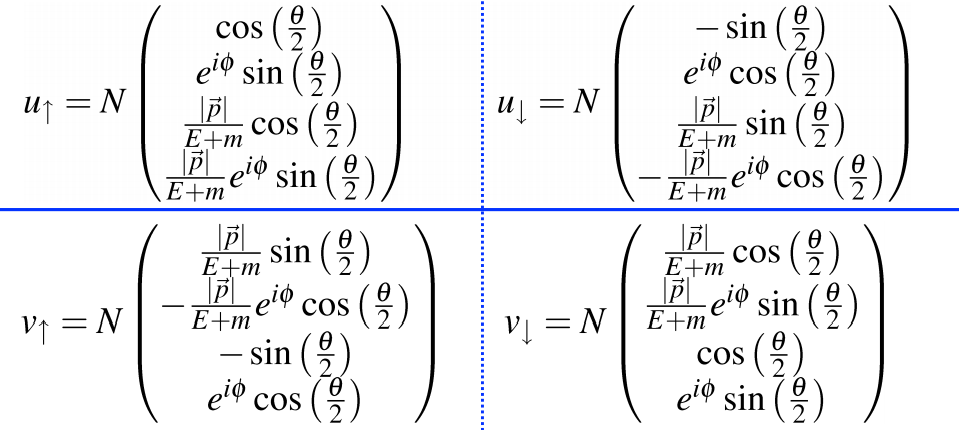
\includegraphics[width=0.6\linewidth]{espinores.png}
\end{center}
\caption{Espinores solución a la ecuación de Dirac y autoestados del operador helicidad.}
\label{espinores}
\end{figure}


\begin{figure}[!h]
\begin{center}
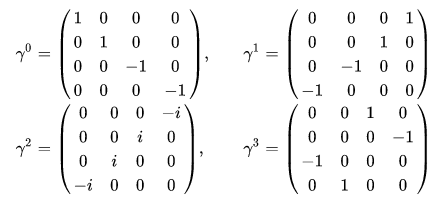
\includegraphics[width=0.6\linewidth]{matrices.png}
\end{center}
\caption{Matrices de Dirac.}
\label{matrices}
\end{figure}






\end{document}
